% SPDX-License-Identifier: MIT
% Usage: \def\lang{zh|en}\def\bleed{0|3} then % SPDX-License-Identifier: MIT
% Usage: \def\lang{zh|en}\def\bleed{0|3} then % SPDX-License-Identifier: MIT
% Usage: \def\lang{zh|en}\def\bleed{0|3} then % SPDX-License-Identifier: MIT
% Usage: \def\lang{zh|en}\def\bleed{0|3} then \input{cover}
\documentclass[UTF8,fontset=fandol]{ctexart}
\usepackage{calc}
\newlength\bl \setlength\bl{\bleed mm}
\usepackage[paperwidth=\dimexpr170mm+2\bl\relax,paperheight=\dimexpr240mm+2\bl\relax,margin=0mm]{geometry}
\usepackage{tikz,xcolor,fontspec}
\setsansfont{texgyreheros-regular.otf}[BoldFont=texgyreheros-bold.otf]
\definecolor{BookTeal}{HTML}{176C68}\definecolor{BookInk}{HTML}{23363E}\definecolor{BookPale}{HTML}{F1F6F5}
\pagestyle{empty}
\begin{document}
\begin{tikzpicture}[remember picture,overlay]
\fill[BookPale] (current page.south west) rectangle (current page.north east);
\node[anchor=south,inner sep=0] at (current page.south) {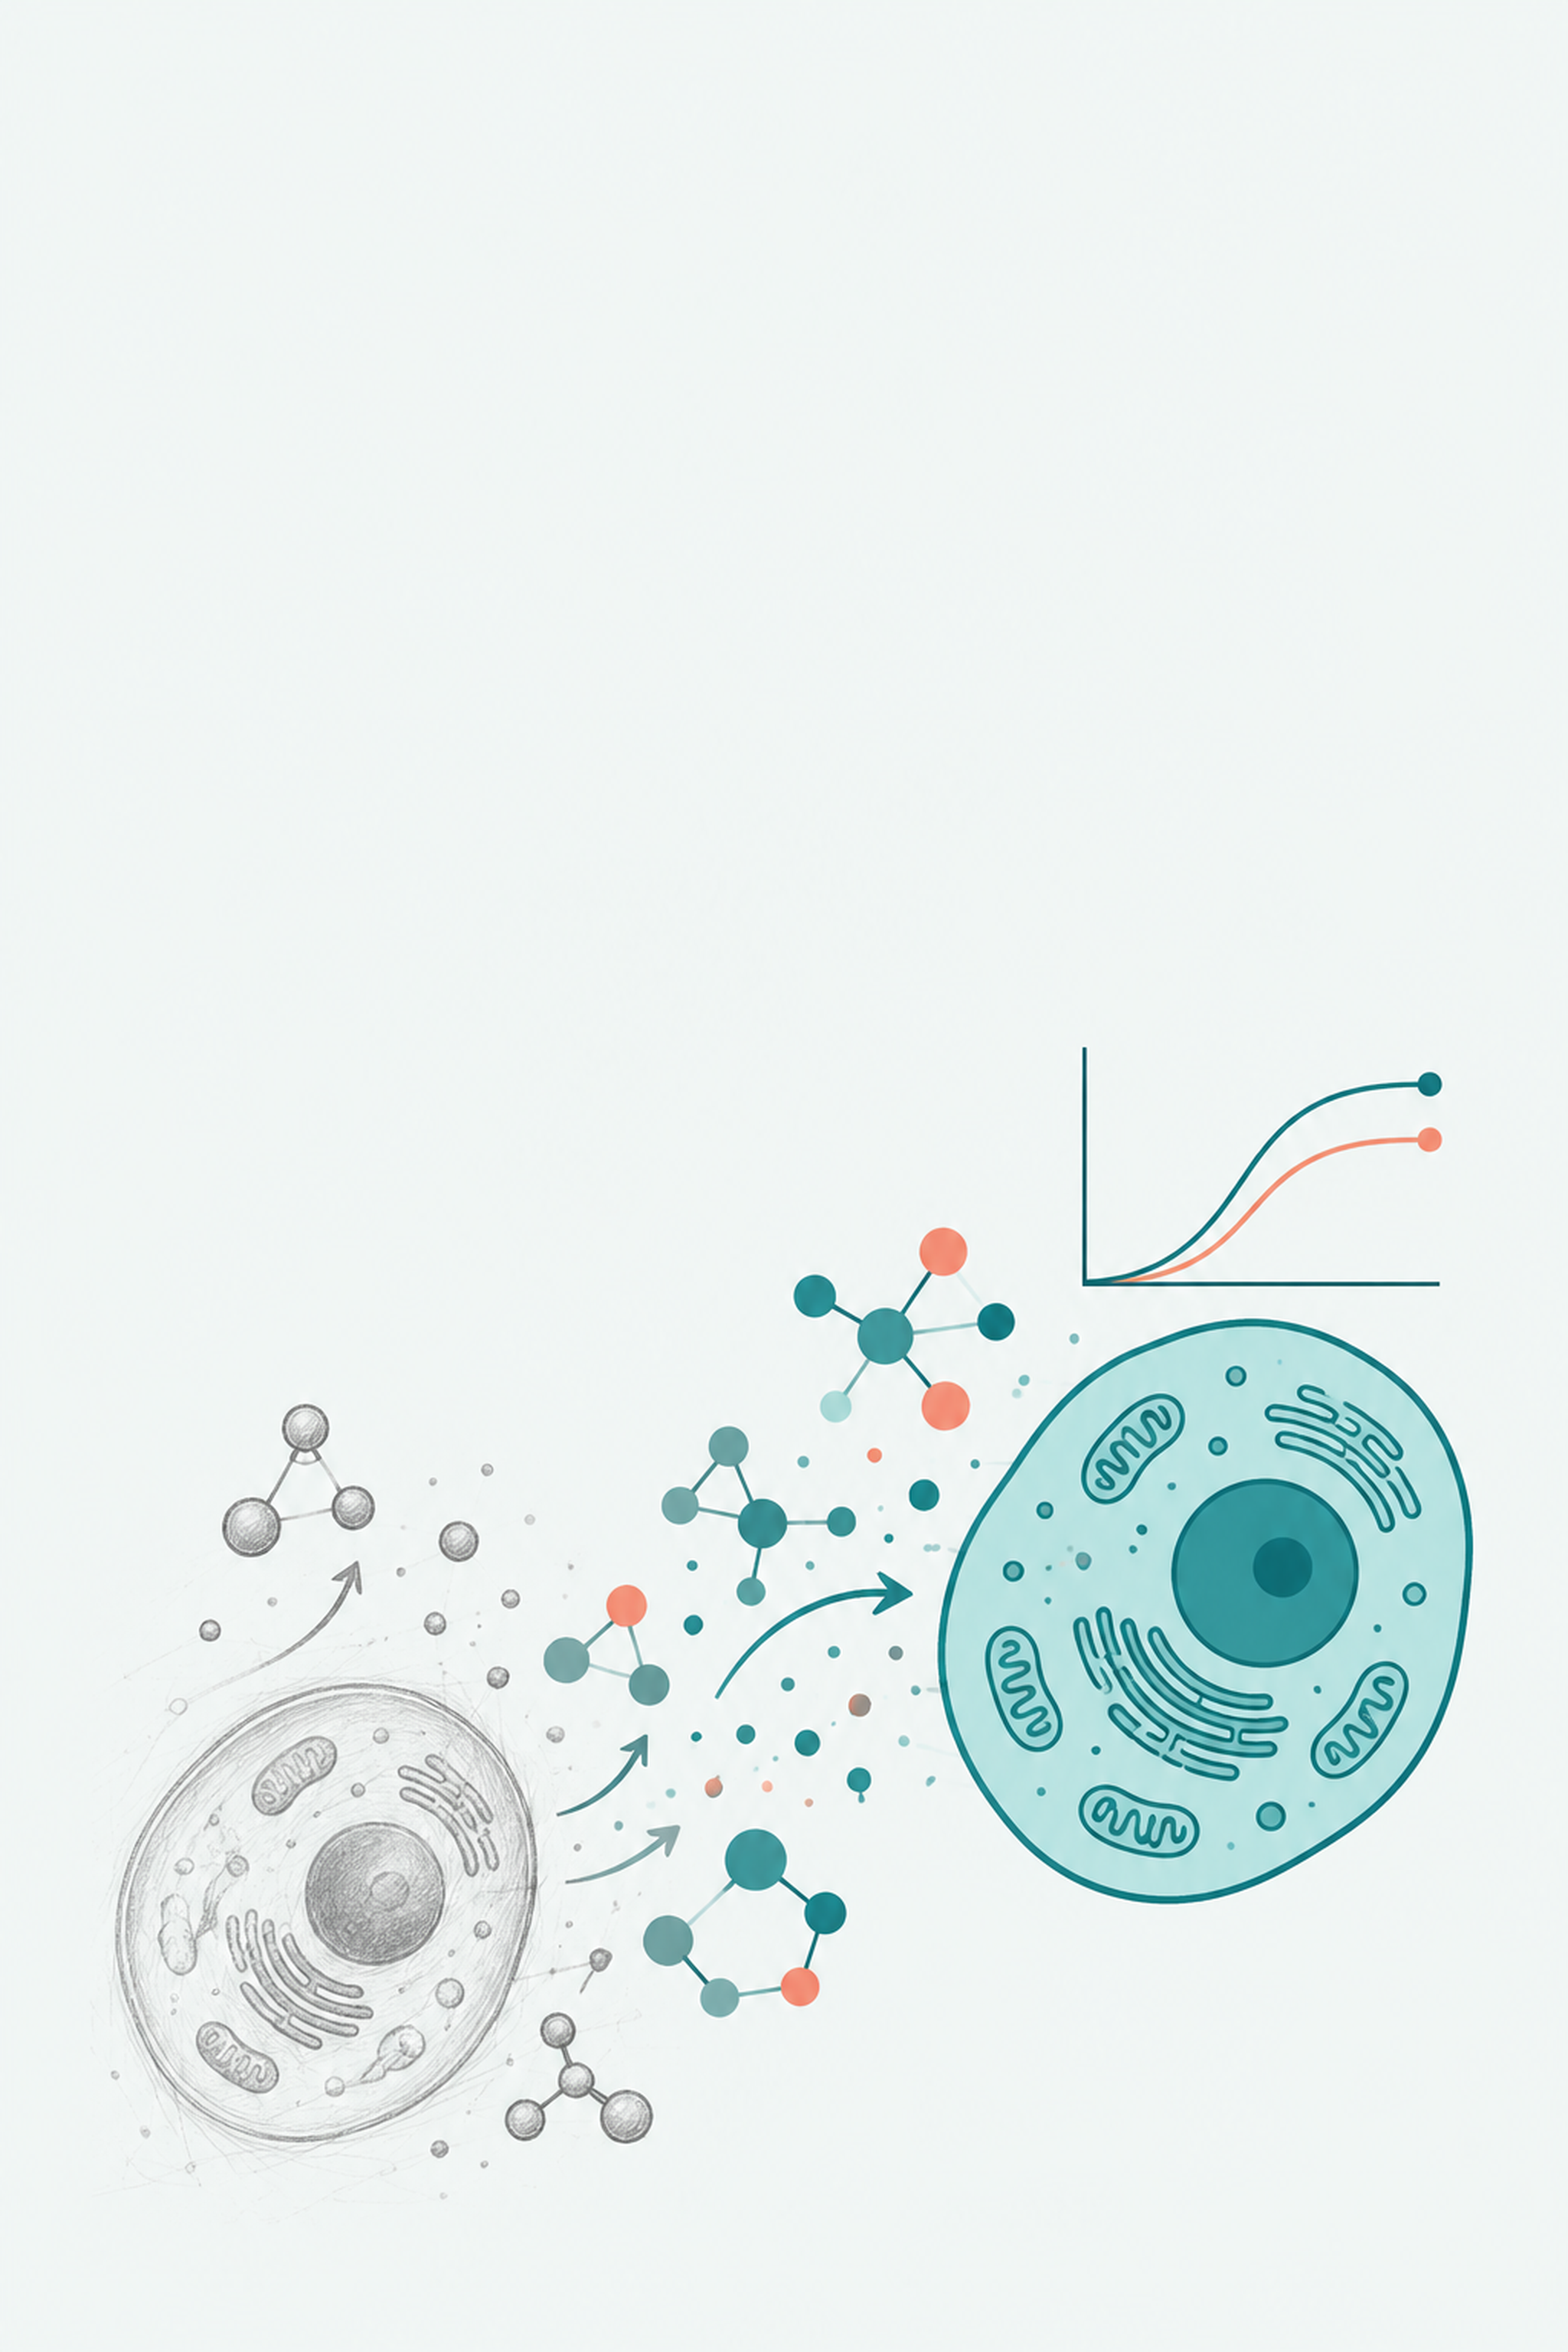
\includegraphics[width=\paperwidth]{../figures/cover/cover-art-a@2x.png}};
\def\L{\dimexpr19mm+\bl\relax}
\def\Tp{\dimexpr-24mm-\bl\relax}
\ifnum\pdfstrcmp{\lang}{zh}=0
\node[anchor=north west,text=BookTeal,font=\sffamily\bfseries\small] at ([xshift=\L,yshift=\Tp]current page.north west) {TopLocalAI 开源书籍 · 以 SciDraw AI 为实践平台};
\draw[BookTeal,line width=1.2pt] ([xshift=\L,yshift=\dimexpr\Tp-8mm\relax]current page.north west) -- ++(18mm,0);
\node[anchor=north west,text=BookInk,font=\bfseries\fontsize{36}{44}\selectfont,align=left,inner sep=0] at ([xshift=\L,yshift=\dimexpr\Tp-15mm\relax]current page.north west) {用 AI\\[2mm]画好科研图};
\node[anchor=north west,text=BookInk,font=\fontsize{15}{20}\selectfont,inner sep=0] at ([xshift=\L,yshift=\dimexpr\Tp-58mm\relax]current page.north west) {从研究思路到论文配图};
\node[anchor=north west,text=BookTeal,font=\sffamily\fontsize{10}{13}\selectfont,inner sep=0] at ([xshift=\L,yshift=\dimexpr\Tp-67mm\relax]current page.north west) {Use AI to Make Better Scientific Figures};
\else
\node[anchor=north west,text=BookTeal,font=\sffamily\bfseries\small] at ([xshift=\L,yshift=\Tp]current page.north west) {An open book by TopLocalAI · Practised with SciDraw AI};
\draw[BookTeal,line width=1.2pt] ([xshift=\L,yshift=\dimexpr\Tp-8mm\relax]current page.north west) -- ++(18mm,0);
\node[anchor=north west,text=BookInk,font=\sffamily\bfseries\fontsize{30}{35}\selectfont,align=left,inner sep=0] at ([xshift=\L,yshift=\dimexpr\Tp-15mm\relax]current page.north west) {Use AI to Make\\Better Scientific\\Figures};
\node[anchor=north west,text=BookInk,font=\sffamily\fontsize{14}{18}\selectfont,inner sep=0] at ([xshift=\L,yshift=\dimexpr\Tp-73mm\relax]current page.north west) {From Research Ideas to Paper Figures};
\fi
\node[anchor=south west,text=BookInk,font=\sffamily\small,inner sep=0] at ([xshift=\L,yshift=\dimexpr14mm+\bl\relax]current page.south west) {TopLocalAI contributors};
\end{tikzpicture}
\end{document}

\documentclass[UTF8,fontset=fandol]{ctexart}
\usepackage{calc}
\newlength\bl \setlength\bl{\bleed mm}
\usepackage[paperwidth=\dimexpr170mm+2\bl\relax,paperheight=\dimexpr240mm+2\bl\relax,margin=0mm]{geometry}
\usepackage{tikz,xcolor,fontspec}
\setsansfont{texgyreheros-regular.otf}[BoldFont=texgyreheros-bold.otf]
\definecolor{BookTeal}{HTML}{176C68}\definecolor{BookInk}{HTML}{23363E}\definecolor{BookPale}{HTML}{F1F6F5}
\pagestyle{empty}
\begin{document}
\begin{tikzpicture}[remember picture,overlay]
\fill[BookPale] (current page.south west) rectangle (current page.north east);
\node[anchor=south,inner sep=0] at (current page.south) {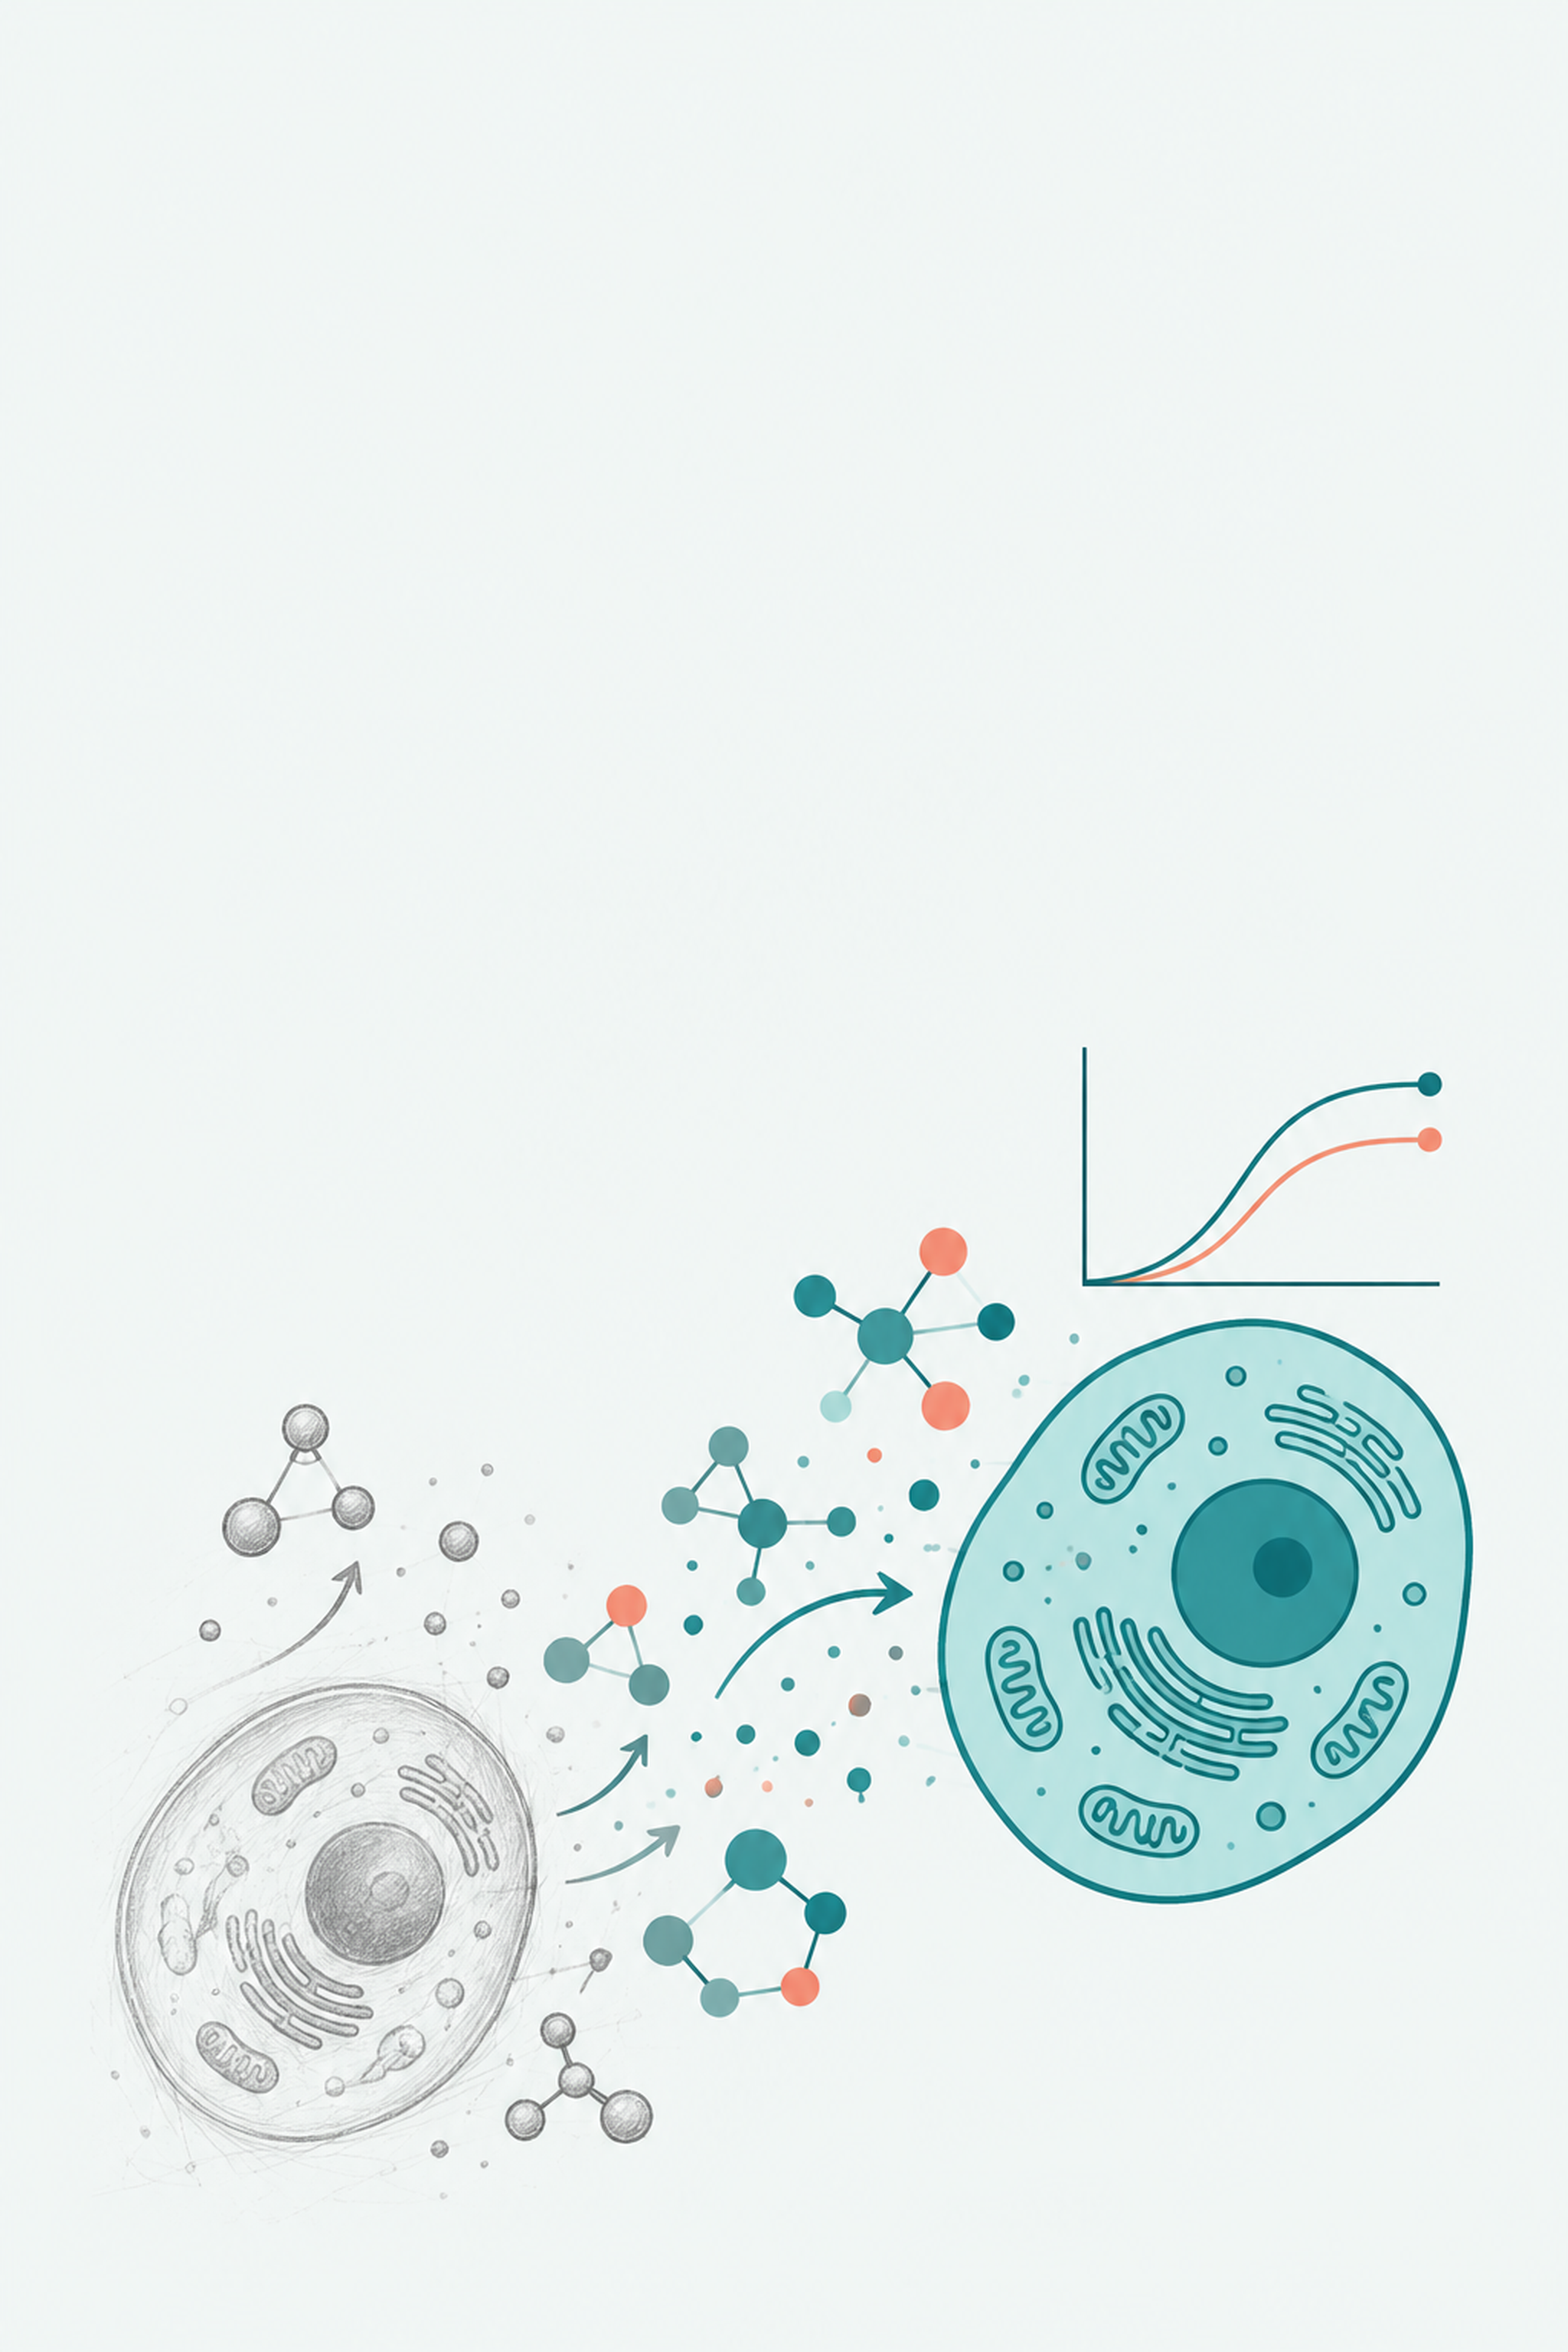
\includegraphics[width=\paperwidth]{../figures/cover/cover-art-a@2x.png}};
\def\L{\dimexpr19mm+\bl\relax}
\def\Tp{\dimexpr-24mm-\bl\relax}
\ifnum\pdfstrcmp{\lang}{zh}=0
\node[anchor=north west,text=BookTeal,font=\sffamily\bfseries\small] at ([xshift=\L,yshift=\Tp]current page.north west) {TopLocalAI 开源书籍 · 以 SciDraw AI 为实践平台};
\draw[BookTeal,line width=1.2pt] ([xshift=\L,yshift=\dimexpr\Tp-8mm\relax]current page.north west) -- ++(18mm,0);
\node[anchor=north west,text=BookInk,font=\bfseries\fontsize{36}{44}\selectfont,align=left,inner sep=0] at ([xshift=\L,yshift=\dimexpr\Tp-15mm\relax]current page.north west) {用 AI\\[2mm]画好科研图};
\node[anchor=north west,text=BookInk,font=\fontsize{15}{20}\selectfont,inner sep=0] at ([xshift=\L,yshift=\dimexpr\Tp-58mm\relax]current page.north west) {从研究思路到论文配图};
\node[anchor=north west,text=BookTeal,font=\sffamily\fontsize{10}{13}\selectfont,inner sep=0] at ([xshift=\L,yshift=\dimexpr\Tp-67mm\relax]current page.north west) {Use AI to Make Better Scientific Figures};
\else
\node[anchor=north west,text=BookTeal,font=\sffamily\bfseries\small] at ([xshift=\L,yshift=\Tp]current page.north west) {An open book by TopLocalAI · Practised with SciDraw AI};
\draw[BookTeal,line width=1.2pt] ([xshift=\L,yshift=\dimexpr\Tp-8mm\relax]current page.north west) -- ++(18mm,0);
\node[anchor=north west,text=BookInk,font=\sffamily\bfseries\fontsize{30}{35}\selectfont,align=left,inner sep=0] at ([xshift=\L,yshift=\dimexpr\Tp-15mm\relax]current page.north west) {Use AI to Make\\Better Scientific\\Figures};
\node[anchor=north west,text=BookInk,font=\sffamily\fontsize{14}{18}\selectfont,inner sep=0] at ([xshift=\L,yshift=\dimexpr\Tp-73mm\relax]current page.north west) {From Research Ideas to Paper Figures};
\fi
\node[anchor=south west,text=BookInk,font=\sffamily\small,inner sep=0] at ([xshift=\L,yshift=\dimexpr14mm+\bl\relax]current page.south west) {TopLocalAI contributors};
\end{tikzpicture}
\end{document}

\documentclass[UTF8,fontset=fandol]{ctexart}
\usepackage{calc}
\newlength\bl \setlength\bl{\bleed mm}
\usepackage[paperwidth=\dimexpr170mm+2\bl\relax,paperheight=\dimexpr240mm+2\bl\relax,margin=0mm]{geometry}
\usepackage{tikz,xcolor,fontspec}
\setsansfont{texgyreheros-regular.otf}[BoldFont=texgyreheros-bold.otf]
\definecolor{BookTeal}{HTML}{176C68}\definecolor{BookInk}{HTML}{23363E}\definecolor{BookPale}{HTML}{F1F6F5}
\pagestyle{empty}
\begin{document}
\begin{tikzpicture}[remember picture,overlay]
\fill[BookPale] (current page.south west) rectangle (current page.north east);
\node[anchor=south,inner sep=0] at (current page.south) {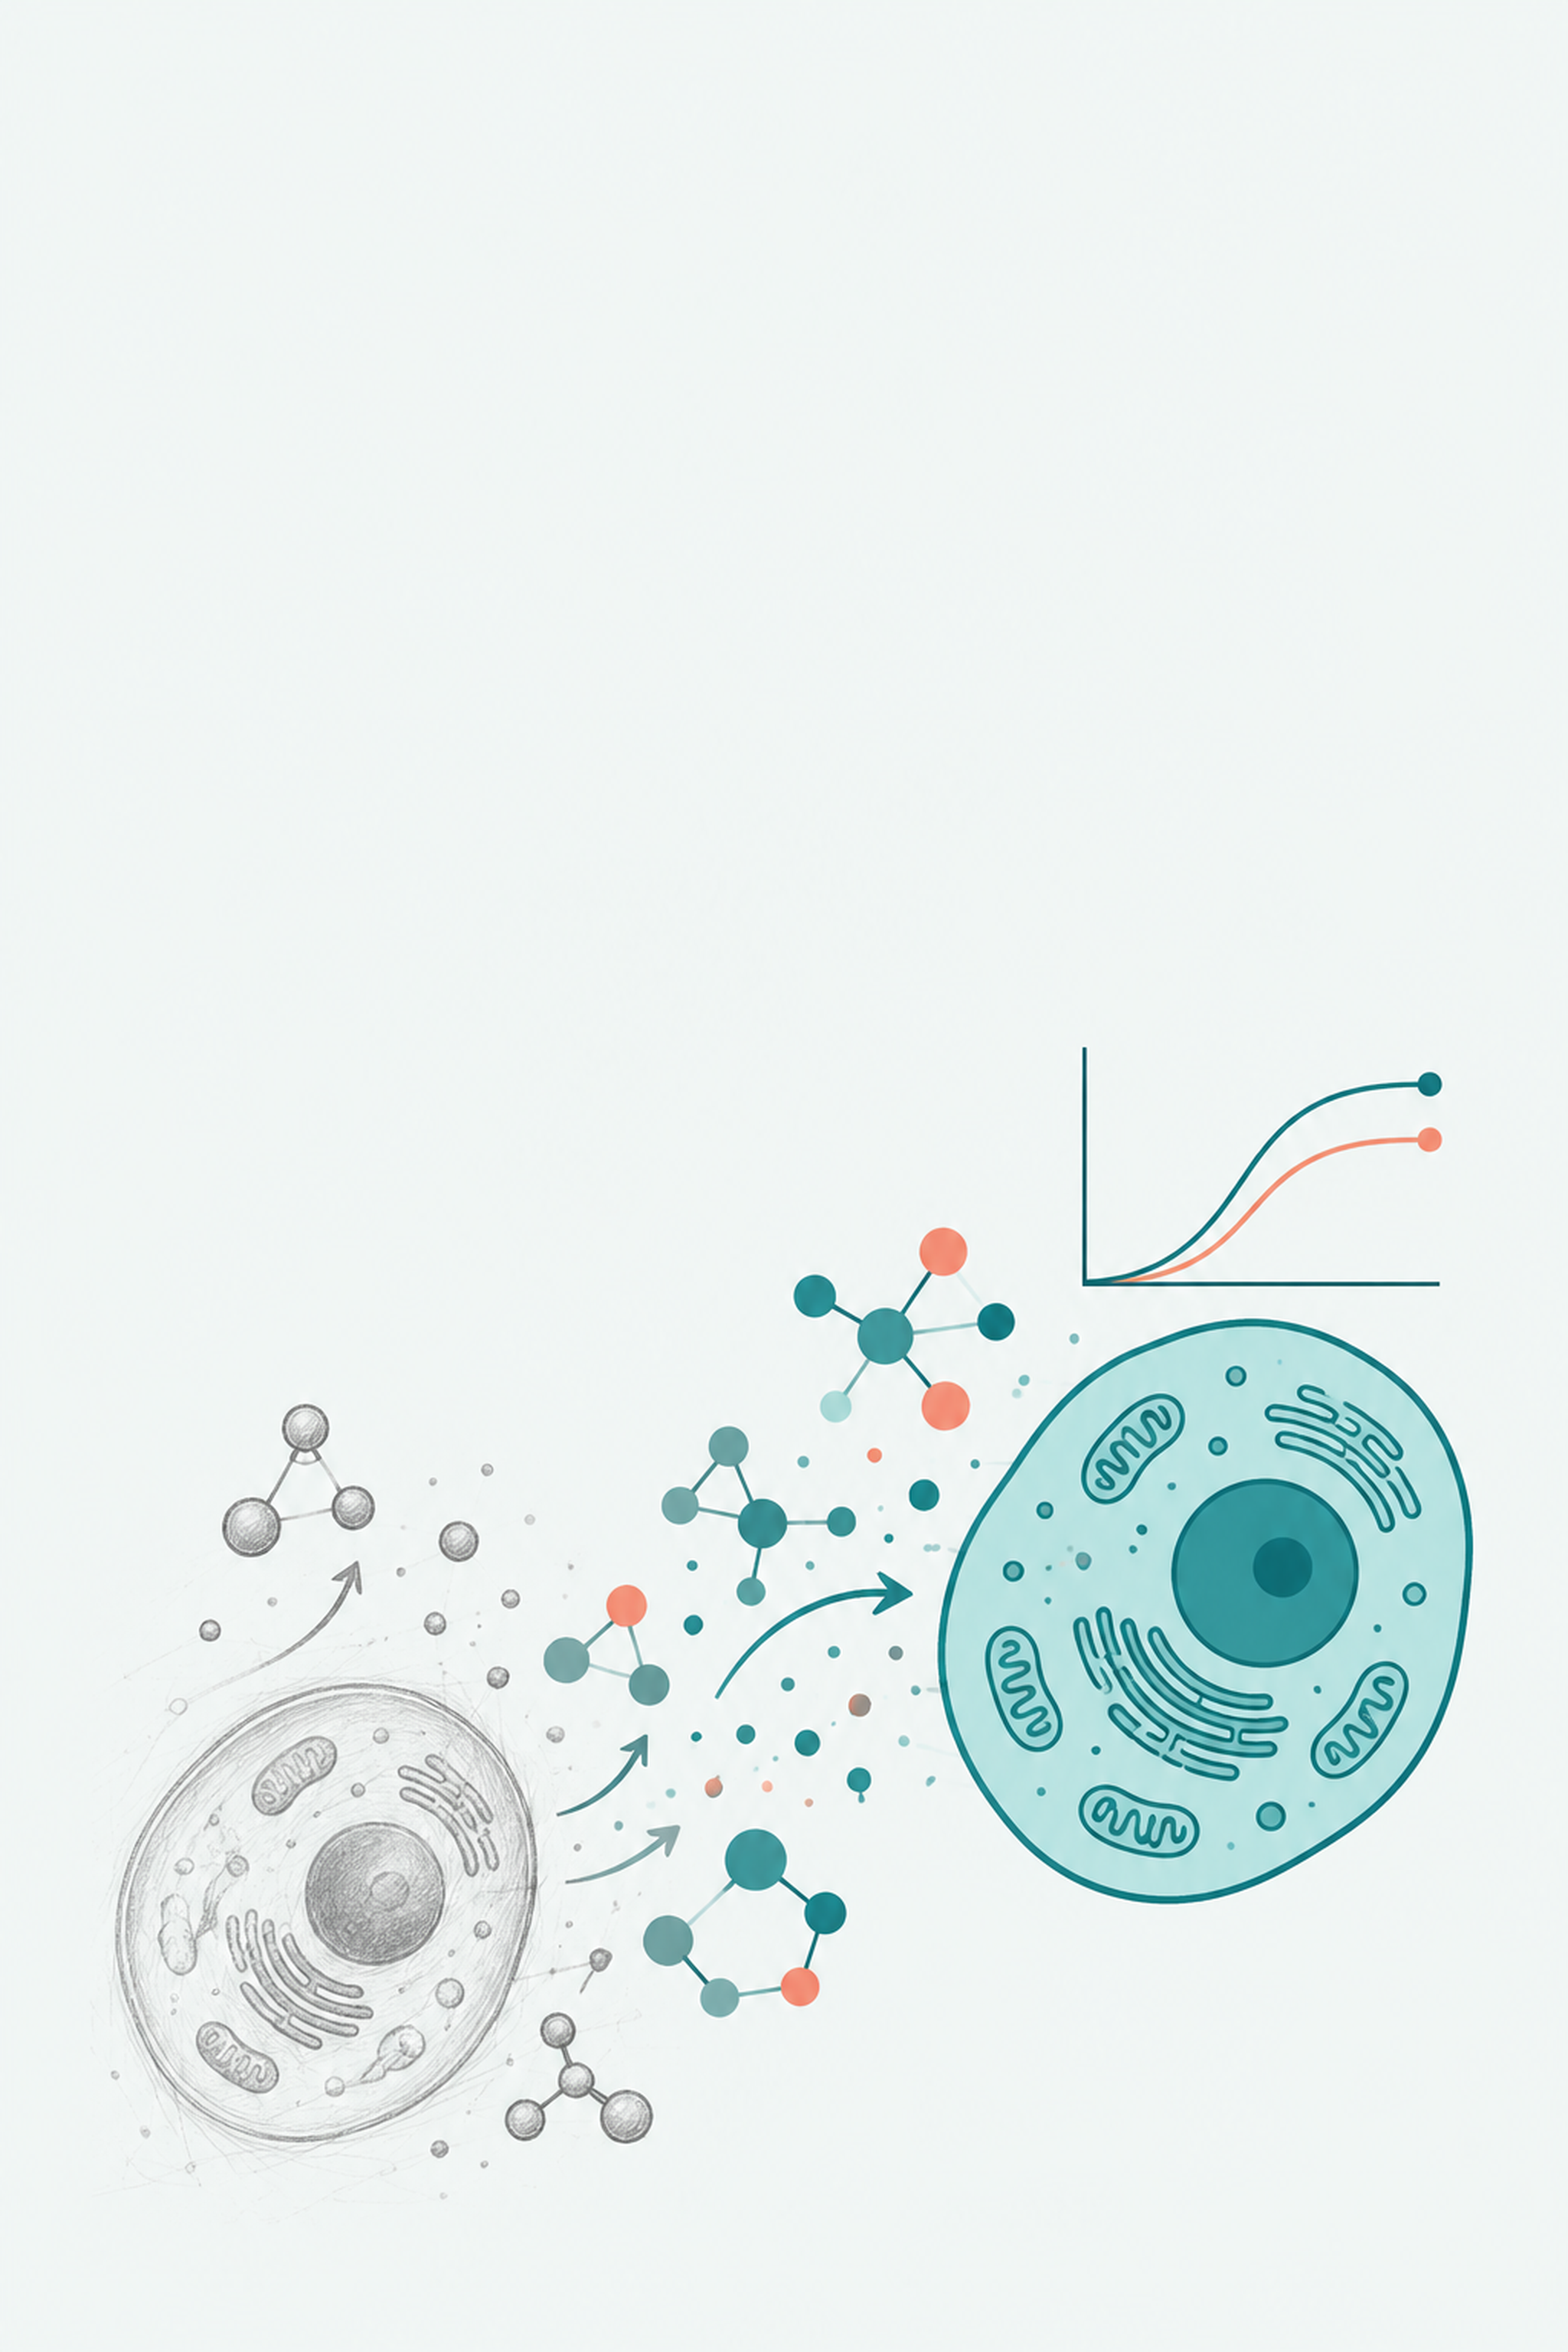
\includegraphics[width=\paperwidth]{../figures/cover/cover-art-a@2x.png}};
\def\L{\dimexpr19mm+\bl\relax}
\def\Tp{\dimexpr-24mm-\bl\relax}
\ifnum\pdfstrcmp{\lang}{zh}=0
\node[anchor=north west,text=BookTeal,font=\sffamily\bfseries\small] at ([xshift=\L,yshift=\Tp]current page.north west) {TopLocalAI 开源书籍 · 以 SciDraw AI 为实践平台};
\draw[BookTeal,line width=1.2pt] ([xshift=\L,yshift=\dimexpr\Tp-8mm\relax]current page.north west) -- ++(18mm,0);
\node[anchor=north west,text=BookInk,font=\bfseries\fontsize{36}{44}\selectfont,align=left,inner sep=0] at ([xshift=\L,yshift=\dimexpr\Tp-15mm\relax]current page.north west) {用 AI\\[2mm]画好科研图};
\node[anchor=north west,text=BookInk,font=\fontsize{15}{20}\selectfont,inner sep=0] at ([xshift=\L,yshift=\dimexpr\Tp-58mm\relax]current page.north west) {从研究思路到论文配图};
\node[anchor=north west,text=BookTeal,font=\sffamily\fontsize{10}{13}\selectfont,inner sep=0] at ([xshift=\L,yshift=\dimexpr\Tp-67mm\relax]current page.north west) {Use AI to Make Better Scientific Figures};
\else
\node[anchor=north west,text=BookTeal,font=\sffamily\bfseries\small] at ([xshift=\L,yshift=\Tp]current page.north west) {An open book by TopLocalAI · Practised with SciDraw AI};
\draw[BookTeal,line width=1.2pt] ([xshift=\L,yshift=\dimexpr\Tp-8mm\relax]current page.north west) -- ++(18mm,0);
\node[anchor=north west,text=BookInk,font=\sffamily\bfseries\fontsize{30}{35}\selectfont,align=left,inner sep=0] at ([xshift=\L,yshift=\dimexpr\Tp-15mm\relax]current page.north west) {Use AI to Make\\Better Scientific\\Figures};
\node[anchor=north west,text=BookInk,font=\sffamily\fontsize{14}{18}\selectfont,inner sep=0] at ([xshift=\L,yshift=\dimexpr\Tp-73mm\relax]current page.north west) {From Research Ideas to Paper Figures};
\fi
\node[anchor=south west,text=BookInk,font=\sffamily\small,inner sep=0] at ([xshift=\L,yshift=\dimexpr14mm+\bl\relax]current page.south west) {TopLocalAI contributors};
\end{tikzpicture}
\end{document}

\documentclass[UTF8,fontset=fandol]{ctexart}
\usepackage{calc}
\newlength\bl \setlength\bl{\bleed mm}
\usepackage[paperwidth=\dimexpr170mm+2\bl\relax,paperheight=\dimexpr240mm+2\bl\relax,margin=0mm]{geometry}
\usepackage{tikz,xcolor,fontspec}
\setsansfont{texgyreheros-regular.otf}[BoldFont=texgyreheros-bold.otf]
\definecolor{BookTeal}{HTML}{176C68}\definecolor{BookInk}{HTML}{23363E}\definecolor{BookPale}{HTML}{F1F6F5}
\pagestyle{empty}
\begin{document}
\begin{tikzpicture}[remember picture,overlay]
\fill[BookPale] (current page.south west) rectangle (current page.north east);
\node[anchor=south,inner sep=0] at (current page.south) {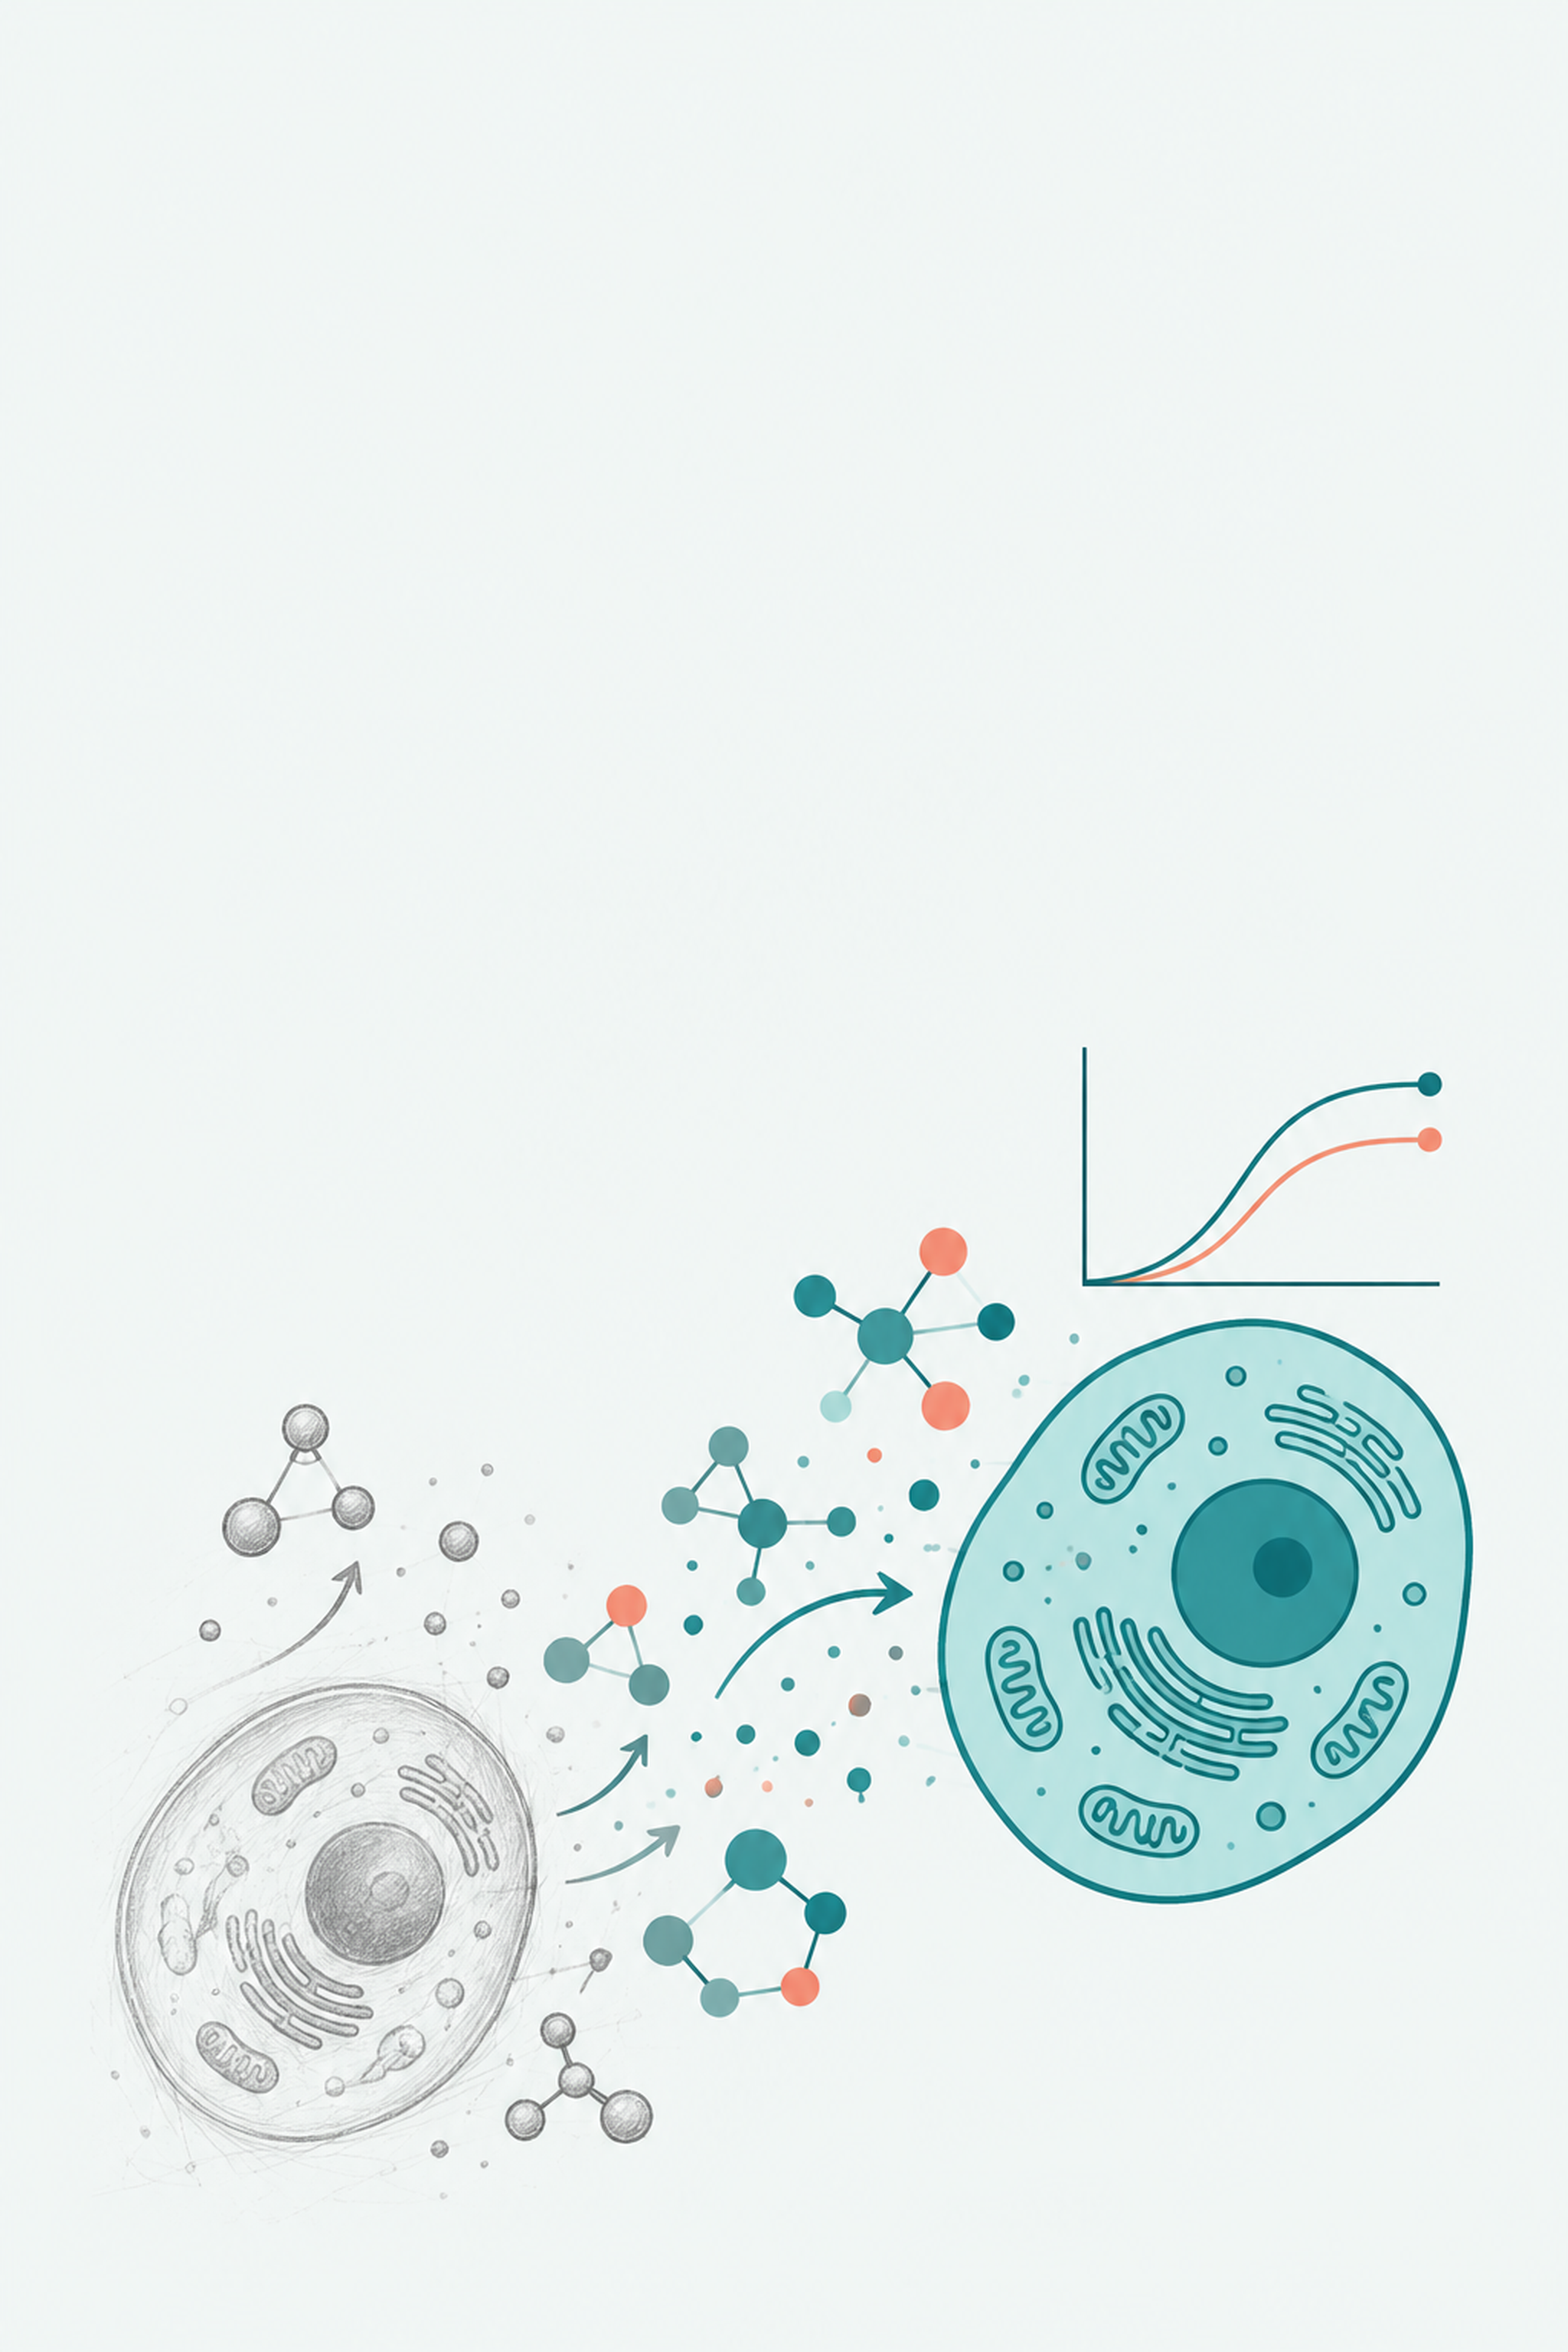
\includegraphics[width=\paperwidth]{../figures/cover/cover-art-a@2x.png}};
\def\L{\dimexpr19mm+\bl\relax}
\def\Tp{\dimexpr-24mm-\bl\relax}
\ifnum\pdfstrcmp{\lang}{zh}=0
\node[anchor=north west,text=BookTeal,font=\sffamily\bfseries\small] at ([xshift=\L,yshift=\Tp]current page.north west) {TopLocalAI 开源书籍 · 以 SciDraw AI 为实践平台};
\draw[BookTeal,line width=1.2pt] ([xshift=\L,yshift=\dimexpr\Tp-8mm\relax]current page.north west) -- ++(18mm,0);
\node[anchor=north west,text=BookInk,font=\bfseries\fontsize{36}{44}\selectfont,align=left,inner sep=0] at ([xshift=\L,yshift=\dimexpr\Tp-15mm\relax]current page.north west) {用 AI\\[2mm]画好科研图};
\node[anchor=north west,text=BookInk,font=\fontsize{15}{20}\selectfont,inner sep=0] at ([xshift=\L,yshift=\dimexpr\Tp-58mm\relax]current page.north west) {从研究思路到论文配图};
\node[anchor=north west,text=BookTeal,font=\sffamily\fontsize{10}{13}\selectfont,inner sep=0] at ([xshift=\L,yshift=\dimexpr\Tp-67mm\relax]current page.north west) {Use AI to Make Better Scientific Figures};
\else
\node[anchor=north west,text=BookTeal,font=\sffamily\bfseries\small] at ([xshift=\L,yshift=\Tp]current page.north west) {An open book by TopLocalAI · Practised with SciDraw AI};
\draw[BookTeal,line width=1.2pt] ([xshift=\L,yshift=\dimexpr\Tp-8mm\relax]current page.north west) -- ++(18mm,0);
\node[anchor=north west,text=BookInk,font=\sffamily\bfseries\fontsize{30}{35}\selectfont,align=left,inner sep=0] at ([xshift=\L,yshift=\dimexpr\Tp-15mm\relax]current page.north west) {Use AI to Make\\Better Scientific\\Figures};
\node[anchor=north west,text=BookInk,font=\sffamily\fontsize{14}{18}\selectfont,inner sep=0] at ([xshift=\L,yshift=\dimexpr\Tp-73mm\relax]current page.north west) {From Research Ideas to Paper Figures};
\fi
\node[anchor=south west,text=BookInk,font=\sffamily\small,inner sep=0] at ([xshift=\L,yshift=\dimexpr14mm+\bl\relax]current page.south west) {TopLocalAI contributors};
\end{tikzpicture}
\end{document}
